%!TEX root = ../TAMUTemplate.tex
%%%%%%%%%%%%%%%%%%%%%%%%%%%%%%%%%%%%%%%%%%%%%%%%%%%
%
%  New template code for TAMU Theses and Dissertations starting Fall 2016.
%
%  Author: Sean Zachary Roberson
%	 Version 3.16.09
%  Last updated 9/12/2016
%
%%%%%%%%%%%%%%%%%%%%%%%%%%%%%%%%%%%%%%%%%%%%%%%%%%%
%%%%%%%%%%%%%%%%%%%%%%%%%%%%%%%%%%%%%%%%%%%%%%%%%%%%%%%%%%%%%%%%%%%%%%
%%                           SECTION V
%%%%%%%%%%%%%%%%%%%%%%%%%%%%%%%%%%%%%%%%%%%%%%%%%%%%%%%%%%%%%%%%%%%%%



\chapter{\texorpdfstring{\uppercase {Higgs Analysis}}{Higgs Analysis}}
\label{ch:analysis}

Data collected by the CMS detector at the LHC is analyzed for the presence of a Higgs boson decaying to the \lvjj final state.
Signal and background Monte Carlo (MC) samples are used to study the efficacy of various object and event selection criteria.
While the signal samples are fully MC based, some of the background samples use data-driven techniques, which will be discussed later in this chapter.
The matrix element probabilities for an event final state being created by a specific diagram are computed.
Several multivariate techniques are studied and used to distinquish between signal-like and background-like events.
We use the discriminator outputs from these mutivariate classifiers to set limits on the SM \HWW cross section.

\section{Data and Monte Carlo Samples}

%The following sections will describe the datasets collected by CMS as well as the MC samples used in this analysis.

\subsection{Data}
\label{sec:data}

As mentioned previously, this analysis makes use of the full 2012 CMS dataset of 8\tev data.
Fig.~\ref{fig:int_lumi_per_day} shows the cumulative delivered, recorded, and validated luminosity versus time.
Only fully validated data, where both the LHC and CMS are completely operational, are use used for CMS analyses~\cite{LumiPublic}.
Table~\ref{tab:dataSamples} shows the data samples used for this analysis, which corresponds to $\sim$19.2\fbinv.
The datasets are split by the two HLT paths used, one which selects for a single high \pt electron and one for a single high \pt muon.
These two separate PDs correspond to the HLT\_Ele27\_WP80\_v* and HLT\_IsoMu24\_eta2p1\_v* trigger paths, respectively.
The HLT\_Ele27\_WP80\_v* path requires a reconstructed electron with \ptgt{27}\gev along with several other criteria grouped into a working point with 80\% efficiency of selecting true electrons.
The HLT\_IsoMu24\_eta2p1\_v* criteria requires an isolated, reconstructed muon with \ptgt{24}\gev within \absetalt{2.1}.
The luminosities listed in the table are associated with a 2.6\% uncertainty as specified in~\cite{CMS-PAS-LUM-12-001} and were collected using the HF luminosity measurements~\cite{CMS-PAS-LUM-13-001}.

\begin{figure}[!hbt]
    \centering
    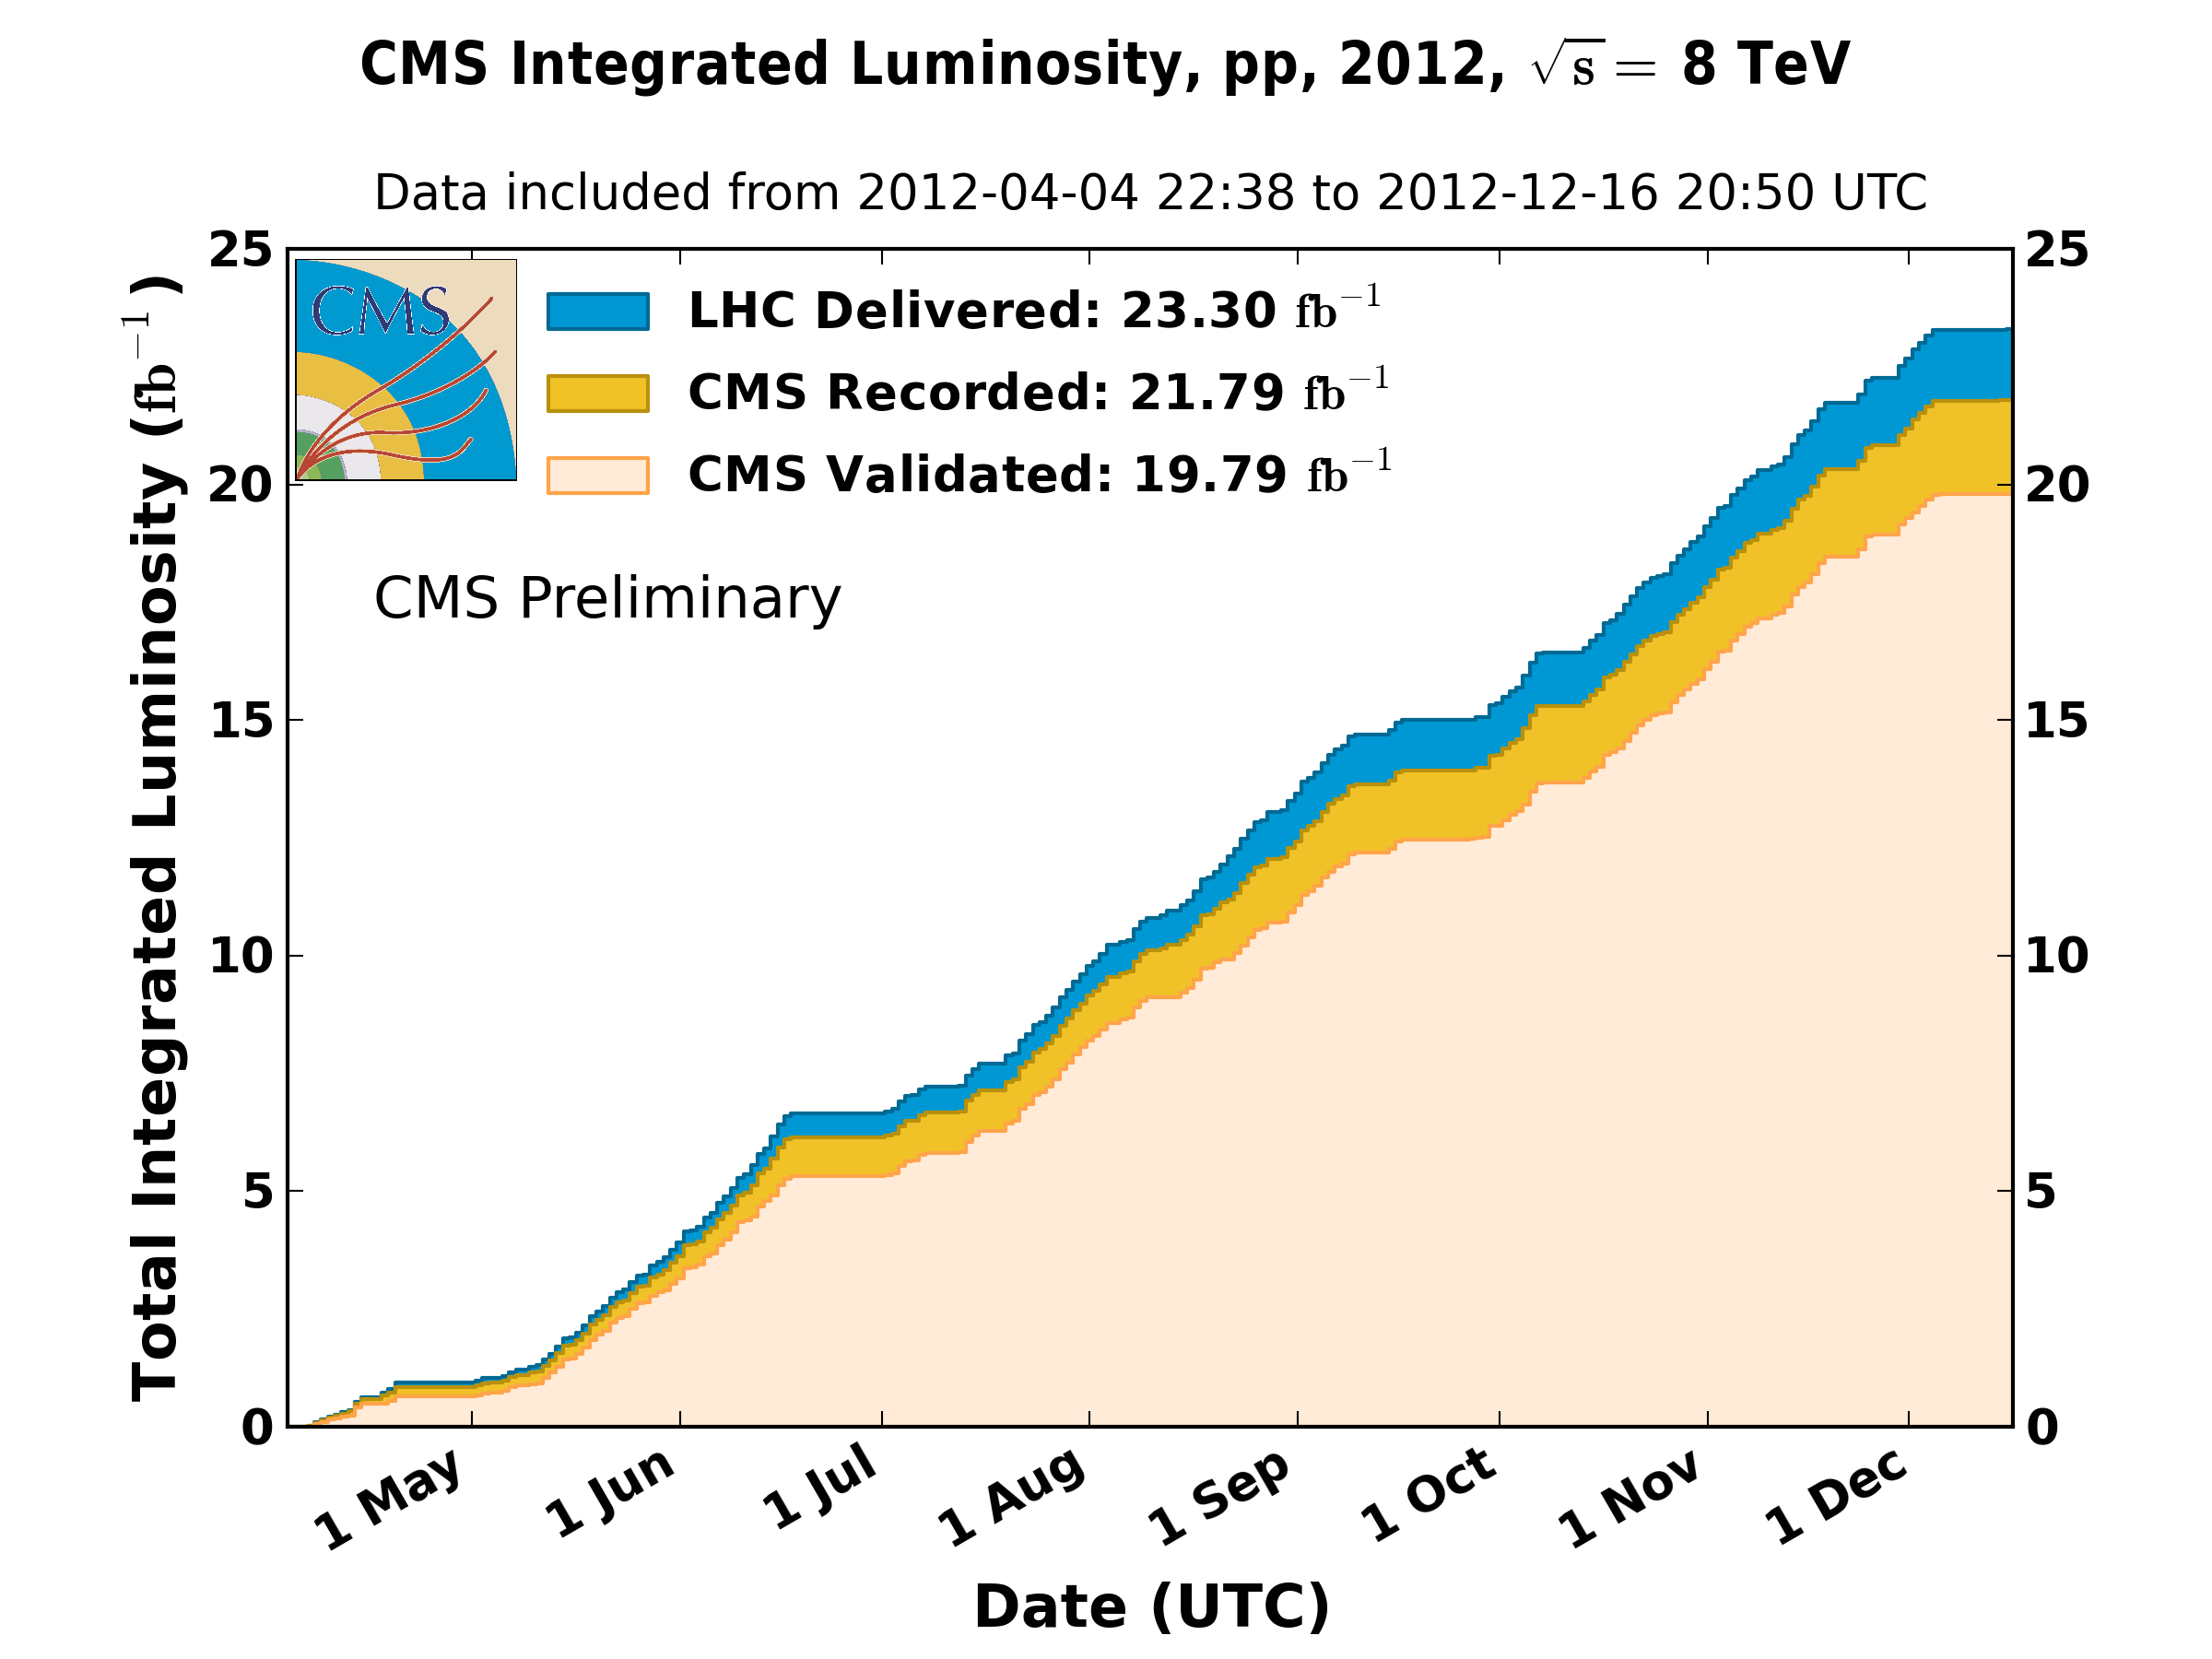
\includegraphics[width=0.95\textwidth]{\figpath/Chapter5/int_lumi_per_day_cumulative_pp_2012_SummerConf.png}
    \caption{Cumulative day-by-day integrated luminosity in 2012 delivered by the LHC (blue), recorded by CMS (dark orange), and validated for physics use (light orange)~\cite{DataQuality}.}
    \label{fig:int_lumi_per_day}
\end{figure}

\begin{table}[hbtp]\footnotesize
\centering
\begin{tabular}{l l l}
\hline
 Dataset & Run Range & Integrated Luminosity \\
\hline
/SingleMu/Run2012A-13Jul2012-v1/AOD & 190645-196531 & 0.809$\fbinv$ \\
/SingleMu/Run2012A-recover-06Aug2012-v1/AOD & 190782-190949 & 0.082$\fbinv$ \\
/SingleMu/Run2012B-13Jul2012-v1/AOD & 193834-196531 & 4.383$\fbinv$ \\
/SingleMu/Run2012C-24Aug2012-v1/AOD & 198022-198523 & 0.489$\fbinv$ \\
/SingleMu/Run2012C-PromptReco-v2/AOD & 194631-203002 & 6.285$\fbinv$ \\
/SingleMu/Run2012D-PromptReco-v1/AOD & 194480-208686 & 7.231$\fbinv$ \\
{\bf Total SingleMu} & {\bf 190645--208686} & {\bf 19.279$\fbinv$} \\
\hline
/SingleElectron/Run2012A-13Jul2012-v1/AOD & 190645-196531 & 0.809$\fbinv$ \\
/SingleElectron/Run2012A-recover-06Aug2012-v1/AOD & 190782-190949 & 0.082$\fbinv$ \\
/SingleElectron/Run2012B-13Jul2012-v1/AOD & 193834-196531 & 4.336$\fbinv$ \\
/SingleElectron/Run2012C-24Aug2012-v1/AOD & 198022-198523 & 0.489$\fbinv$ \\
/SingleElectron/Run2012C-PromptReco-v2/AOD & 194631-203002 & 6.194$\fbinv$ \\
/SingleElectron/Run2012D-PromptReco-v1/AOD & 194480-208686 & 7.238$\fbinv$\\
{\bf Total SingleElectron} & {\bf 190645--208686} & {\bf 19.148$\fbinv$} \\
\hline
\end{tabular}
\caption{The datasets analyzed for this analysis.}
\label{tab:dataSamples}
\end{table}

\subsection{Monte Carlo}

This analysis makes use of MC simulation to study the background processes which have similar final states to that of the \HWWlvjj signal.
Both the kinematic distributions and the final yields are extracted from these samples.
The MC simulation is used for all beckgrounds except for the multijet process, where a data-driven approach is used instead.
The process of developing this sample is described in detail in the section~\ref{sec:QCD_data-driven_sample}.
The signal sample kinematics and yields are also taken from MC.
Tables~\ref{tab:SignalSamples} and~\ref{tab:bkgSamples} list all of the MC sample for the Higgs signals and SM background processes, respectively.
The SM background and volunteer signal samples are centrally produced by the CMS collaboration.
The \ggH samples were produced specifically for this analysis.
All of the samples, reguardless of who produced them, are stored in a database called the Data Aggregation System (DAS) and organized by the ``Dataset Name'' field.
The backgrounds were modeled by MC samples generated with \textsc{MadGraph}~\cite{Alwall:2014hca} and \textsc{pythia6}~\cite{1126-6708-2006-05-026}. 
The signal MC samples were also generated by \textsc{pythia6}.
Tables~\ref{tab:bkgSamples} and~\ref{tab:SignalSamples} list all of the MC for the Higgs signal and SM background processes, respectively.

\begin{sidewaystable}[hbtp]\footnotesize
\centering
\begin{tabular}{l p{0.50\textwidth} l l}
\hline
\multicolumn{4}{c}{Signal Processes} \\
\hline
Production \& Decay Modes & Dataset Name & Cross Section [\unit{pb}] & BR\\  \hline
\ggH; $\MH=\text{125}\gev$, \HWWlvjj & /LQ-ggh125\_BIG\_SIM\_ggH125\_part1/aperloff-LQ-ggh125\_AODSIM\_Summer12\_START53\_V7E-{\newline}768a14b04b0ac2af0d20e6783fbdb759/USER & 19.27 & 0.0947 \\
  & /LQ-ggh125\_BIG\_GEN\_part2/aperloff-LQ-ggh125\_BIG\_RECO\_part2-33e909ff21293ad9fa8564de2959fe54/USER & 19.27 & 0.0947\\
  & /LQ-ggh125\_BIG\_GEN\_part3/aperloff-LQ-ggh125\_BIG\_RECO\_part3-33e909ff21293ad9fa8564de2959fe54/USER & 19.27 & 0.0947\\
  & /LQ-ggh125\_Part6\_SIM/goodell-LQ-qqh125\_RECO\_Part6-33e909ff21293ad9fa8564de2959fe54/USER & 19.27 & 0.0947\\
  & /LQ-ggh125\_Part7\_SIM/goodell-LQ-qqh125\_RECO\_Part7-33e909ff21293ad9fa8564de2959fe54/USER & 19.27 & 0.0947\\
  & /LQ-ggh125\_Part8\_GENSIM/goodell-LQ-ggh125\_Part8\_RECO-33e909ff21293ad9fa8564de2959fe54/USER & 19.27 & 0.0947\\
\qqH; $\MH=\text{125}\gev$, \HWWlvjj & /LQ-vbf125\_GENSIM/ajkumar-LQ-qqh125\_AODSIM\_Summer12\_{\newline}START53\_V7A-c8f8ed334db8a7d6f56c62266b1dfa5b/USER & 1.578 & 0.0947\\
\WH, \ZH, \ttH; $\MH=\text{125}\gev$, \HWW, inclusive & /WH\_ZH\_TTH\_HToWW\_M-125\_8TeV-pythia6 & 1.249 & 0.215\\\hline
\multicolumn{4}{c}{Non signal Higgs Production} \\ \hline
\WH, \ZH, \ttH; $\MH=\text{125}\gev$, \HZZ, inclusive & /WH\_ZH\_TTH\_HToZZ\_M-125\_8TeV-pythia6 & 1.249 & 0.0264\\
\WH; $\MH=\text{125}\gev$, \Hbb, \Wlv & /WH\_WToLNu\_HToBB\_M-125\_8TeV-powheg-herwigpp & 0.7046 & 0.1879\\
\ttH; $\MH=\text{125}\gev$, \Hbb & /TTH\_HToBB\_M-125\_8TeV-pythia6 & 0.1293 & 0.577\\
\hline
\end{tabular}
\caption{List of signal datasets and cross sections. All of the centrally produced sample names are followed by /Summer12\_DR53X-PU\_S10\_START53\_V7A-v1/AODSIM.}
\label{tab:SignalSamples}
\end{sidewaystable}

\begin{sidewaystable}[hbtp]\footnotesize
\centering
\begin{tabular}{l p{0.65\textwidth} l}
\hline
\multicolumn{3}{c}{Background Processes} \\
\hline
Process & Dataset Name & Cross Section [\unit{pb}] \\
\hline
\Wjets & /WJetsToLNu\_TuneZ2Star\_8TeV-madgraph-tarball & 37509 \\
\ttbar & /TTJets\_MassiveBinDECAY\_TuneZ2star\_8TeV-madgraph-tauola & 225.197 \\
\Zjets & /DYJetsToLL\_M-50\_TuneZ2Star\_8TeV-madgraph-tarball & 3387.6 \\
\WW & /WW\_TuneZ2star\_8TeV\_pythia6\_tauola & 54.838 \\
\WZ & /WZ\_TuneZ2star\_8TeV\_pythia6\_tauola & 33.21 \\
\ZZ & /ZZ\_TuneZ2star\_8TeV\_pythia6\_tauola & 17.654 \\
$\cPqt\rightarrow\cPqb\ell\nu$ (\cPqs-channel) & /T\_s-channel\_TuneZ2star\_8TeV-powheg-tauola & 3.79 \\
$\cPqt\rightarrow\cPqb\ell\nu$ (\cPqt-channel) & /T\_t-channel\_TuneZ2star\_8TeV-powheg-tauola & 56.4 \\
$\cPqt\rightarrow{X}$ (\cPqt\W-channel) & /T\_tW-channel-DR\_TuneZ2star\_8TeV-powheg-tauola & 11.1 \\
$\cPaqt\rightarrow\cPqb\ell\nu$ (\cPqs-channel) & /Tbar\_s-channel\_TuneZ2star\_8TeV-powheg-tauola & 1.76 \\
$\cPaqt\rightarrow\cPqb\ell\nu$ (\cPqt-channel) & /Tbar\_t-channel\_TuneZ2star\_8TeV-powheg-tauola & 30.7 \\
$\cPaqt\rightarrow{X}$ (\cPqt\W-channel) & /Tbar\_tW-channel-DR\_TuneZ2star\_8TeV-powheg-tauola & 11.1 \\
QCD (\Pe-channel) & See table~\ref{tab:dataSamples} for a list of SingleElectron datasets & N/A \\
QCD (\Pmu-channel) & See table~\ref{tab:dataSamples} for a list of SingleMu datasets & N/A \\
\hline
\end{tabular}
\caption{List of background MC datasets and cross sections used in the analysis. Every dataset name is followed by /Summer12\_DR53X-PU\_S10\_START53\_V7A-v1/AODSIM. In addition to v1, this analysis also uses v2 of the \Wjets sample.}
\label{tab:bkgSamples}
\end{sidewaystable}

The \ttbar, \Wjets, and \Zjets SM background samples are generated using \textsc{Mad}\textsc{Graph} v5.1.3.30~\cite{Alwall:2014hca}.
The \ttbar sample is inclusive, meaning that it includes all decay modes of the \W boson coming from the top decay.
The \Wjets and \Zjets samples are also inclusive, but in this case it means that in addition to the leptonic decay of the boson there are any number of final state jets.
The single top quark samples are modeled using the \textsc{POWHEG} 1.0 r138 ~\cite{POWHEG2,POWHEG:singlet,POWHEG:singletW} generator.
The diboson processes use the \textsc{pythia} v6.4.24 generator~\cite{1126-6708-2006-05-026}.
The cross sections for the \ttbar and single top quark processes are calculated at next-to-next-to-leading logarithmic (NNLL) accuracy~\cite{TOPCrossSec} while the inclusive \Wjets and \Zjets processes are calculated at next-to-next-to-leading order (NNLO) accuracy~\cite{FEWZ}.
The diboson cross sections are calculated at next-to-leading order (NLO) accuracy~\cite{MCFM}.

The \HWW signal samples are generated with \textsc{pythia} v6.4.24~\cite{1126-6708-2006-05-026}, where one \W is required to decay leptonically while the other is required to decay hadronically.
The cross sections for the Higgs production are calculated at NNLL QCD and NLO EW accuracies.
The calculations for gluon-gluon fusion and VBF production cross sections use the complex-pole-scheme (CPS) while the associated production cross section are calculated with the zero-width-approximation (ZWA)~\cite{Heinemeyer:2013tqa}.
These samples were privately produced because the centrally produces samples did not include enough events and had large statistical fluctuations.

\subsection{Multijet-QCD Background}
\label{sec:QCD_data-driven_sample}

It is well known that the QCD process is difficult to model to the desired level of accuracy.
Additionally, the event selection in this analysis requires two isolated jets and an isolated lepton, which vastly reduces the number of QCD MC events that pass the selection criteria.
Although the probability to mis-reconstruct a jet as a lepton is fairly low, the production cross section for the multijet process is extremely high and thus cannot be ignored.
When using the MC samples we are left with a statistically limited sample that is almost useless for describing this background.

Rather than relying on MC for the QCD background sample, a data-driven sample was created by using the same trigger requirements as the data, but removing the isolation requirement for the lepton and inverting the lepton particle flow isolation cut during selection.
The main idea of the method is to utilize differences in lepton identification properties that separate prompt, isolated leptons from \W and \Z decays, also known as ``real leptons,'' from non-prompt, non-isolated leptons, also known as ``fake leptons.''
The normal signal selection requires an isolated lepton, without other particles around it, to limit this sort of ``fake lepton,'' but this is exactly the type of property we want to select for when forming a QCD sample from data.
This process provides a completely orthogonal sample of QCD events from data that won't, and shouldn't be used for signal extraction.
Since we make use of the entire 2012 dataset\footnote{The QCD events are scaled slightly to account for failed jobs (missing luminosity) during processing.}, we end up with statistically rich samples containing lots of mis-identified leptons.

A complete description of the event selection will be discussed in section~\ref{ch:event_selection}, but here I will just talk about the isolation requirements.
The loosest lepton PF isolation requirement used to determine the signal region is $\pfiso<0.2$, which is used to veto on ``loose'' or questionable leptons.
The assumption is that any lepton with $\pfiso>0.2$ is a mis-reconstructed lepton coming from QCD.
For electrons we must also turn off the MVA-based identification requirements as they are stringent enough that they won't allow for any fake leptons to pass our selection.
As mentioned before, the electrons must still pass the ``HLT\_Ele27\_WP80\_v*'' electron trigger used for the data containing our signal.
On the other hand, the muon trigger is changed to be ``HLT\_Mu24\_eta2p1\_v*'' to remove the isolation requirement that was included in the trigger used to select for the signal.

In order to gain greater separation from the signal selection to ensure as little non-QCD contamination as possible, we actually use a minimum isolation requirement of $\pfiso>0.3$.
We also put an upper limit on the PF isolation value to keep the sample from having a bias towards high nPV values.
For electrons the upper limit was 0.7 and for muons it was 2.0.
The $1\sigma$ systematic uncertainty bands for electrons (muons) were selected to be $0.2<\pfiso<0.3$ on the low side and $>$0.7 (2.0) for the high side
Fig.~\ref{fig:PFIsolation} shows the pf isolation values contained in the electron multijet and data samples as a function of $\eta$.

\begin{figure}[!hbt]
    \centering
    \begin{subfigure}[t]{0.475\textwidth}
        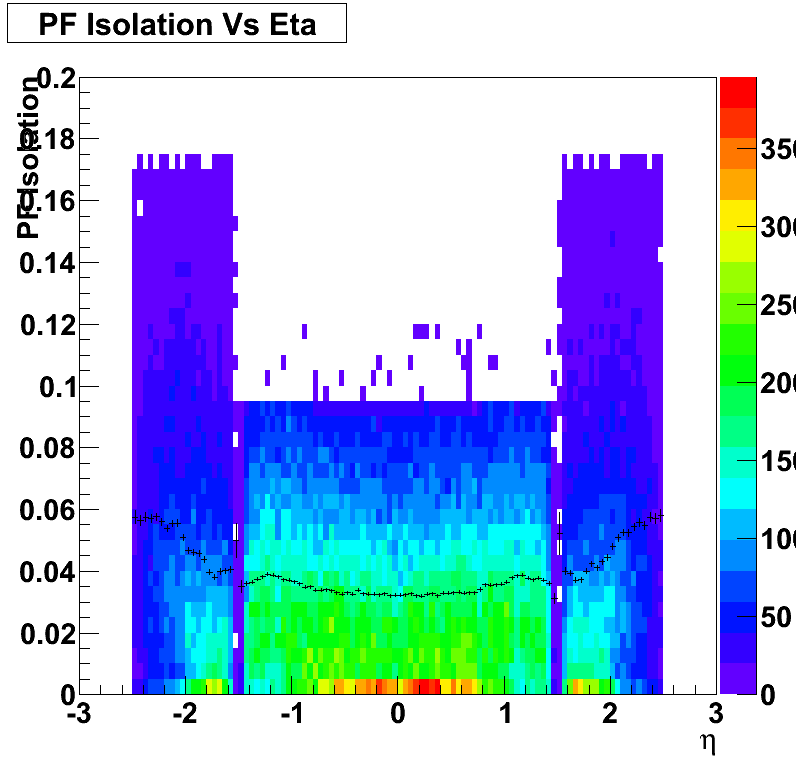
\includegraphics[width=\textwidth]{\figpath/Chapter5/pfIsoVsEta_DATA.png}
        \caption{}
        \label{fig:PFIsolationData}
    \end{subfigure}
    \begin{subfigure}[t]{0.475\textwidth}
        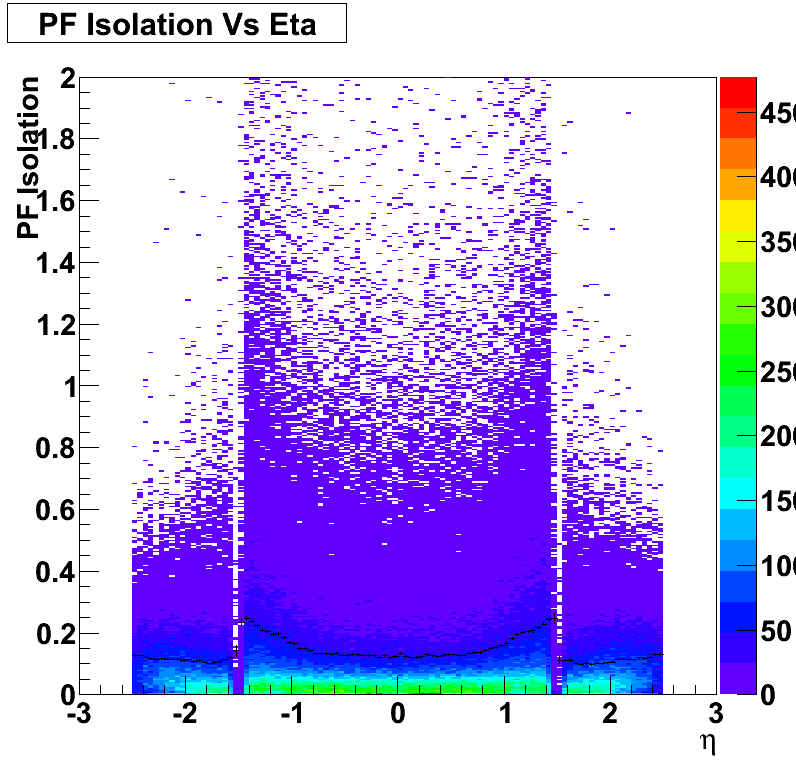
\includegraphics[width=\textwidth]{\figpath/Chapter5/pfIsoVsEta_Full.png}
        \caption{}
        \label{fig:PFIsolationFull}
    \end{subfigure}
    \caption{The PF isolation for the electron channel as a function of $\eta$ (left) with and (right) without the lepton isolation and electron MVA-based identification requirements.}
    \label{fig:PFIsolation}
\end{figure}

\section{Event \& Object Selection}
\label{ch:event_selection}

The reconstruction algorithms described in chapter~\ref{ch:event_reconstruction} are designed to be fairly generic and applicable to a wide array of physics analyses.
Specific groups within CMS called physics object groups (POGs) are responsible for developing object quality criteria which must be implemented by each analysis to prevent fake or poorly reconstructed objects.
This section will discuss the object selection criteria used to identify vertices, electrons, muons, jets, and \VETslash, which all meet or exceed the object requirements as set by the relevant POGs.
Only events which have the right quality and multiplicities of these objects will be used in the analysis.

Like most analyses, this one selects for a single good quality primary vertex, although the presence of additional vertices (pileup) does not disqualify the event.
The primary vertex must pass certain additional quality criteria.
There must be at least four degrees of freedom used to find the vertex, the absolute value of the $z$-coordinate of the vertex must be less than 24\unit{cm}, the absolute value of the $\rho$-coordinate (cylindrical coordinate system) must be less than 2.0\unit{cm}, and the vertex must not be identified as a fake vertex.
These criteria are summarized in table~\ref{tab:vertex_selection}.

\begin{table}[hbtp]\footnotesize
\centering
\begin{tabular}{l l}
\hline
Cut & Value \\
\hline
N\textsubscript{DOF} & $\geqslant$4 \\
$|z|$ & $\leqslant$24\unit{cm} \\
$|\rho|$ & $\leqslant$2.0\unit{cm} \\
\hline
\end{tabular}
\caption{The primary vertex selection requirements for this analysis.}
\label{tab:vertex_selection}
\end{table}

As mentioned before, this analysis selects for the presence of one lepton, either an electron or muon, at least two jets, and some amount of \VETslash.
In practical terms this means that we select for one tight electron (muon) as defined in section~\ref{sec:electrons} (\ref{sec:muons}) and veto the event if there are any additional tight or loose electrons and muons (muons and electrons).
Some additional cuts beyond those of the identification requirements are imposed to cut out some of the background events while maximizing the number of signal events we could use for the multivariate analysis techniques.
The additional \pt and $\eta$ requirements as specified in the same sections are also applied.
For the tight electrons this meant raising the \pt requirement from 27\gev to 30\gev, which avoids using events right on the trigger turn on threshold while only removing $\sim$5\% of signal events, as seen in fig.~\ref{fig:electronPt_signal_loss}. 
Because muon reconstruction and identification in CMS is very good, we only raised the \pt requirement to 25\gev from 24\gev.

\begin{figure}[!hbt]
    \centering
    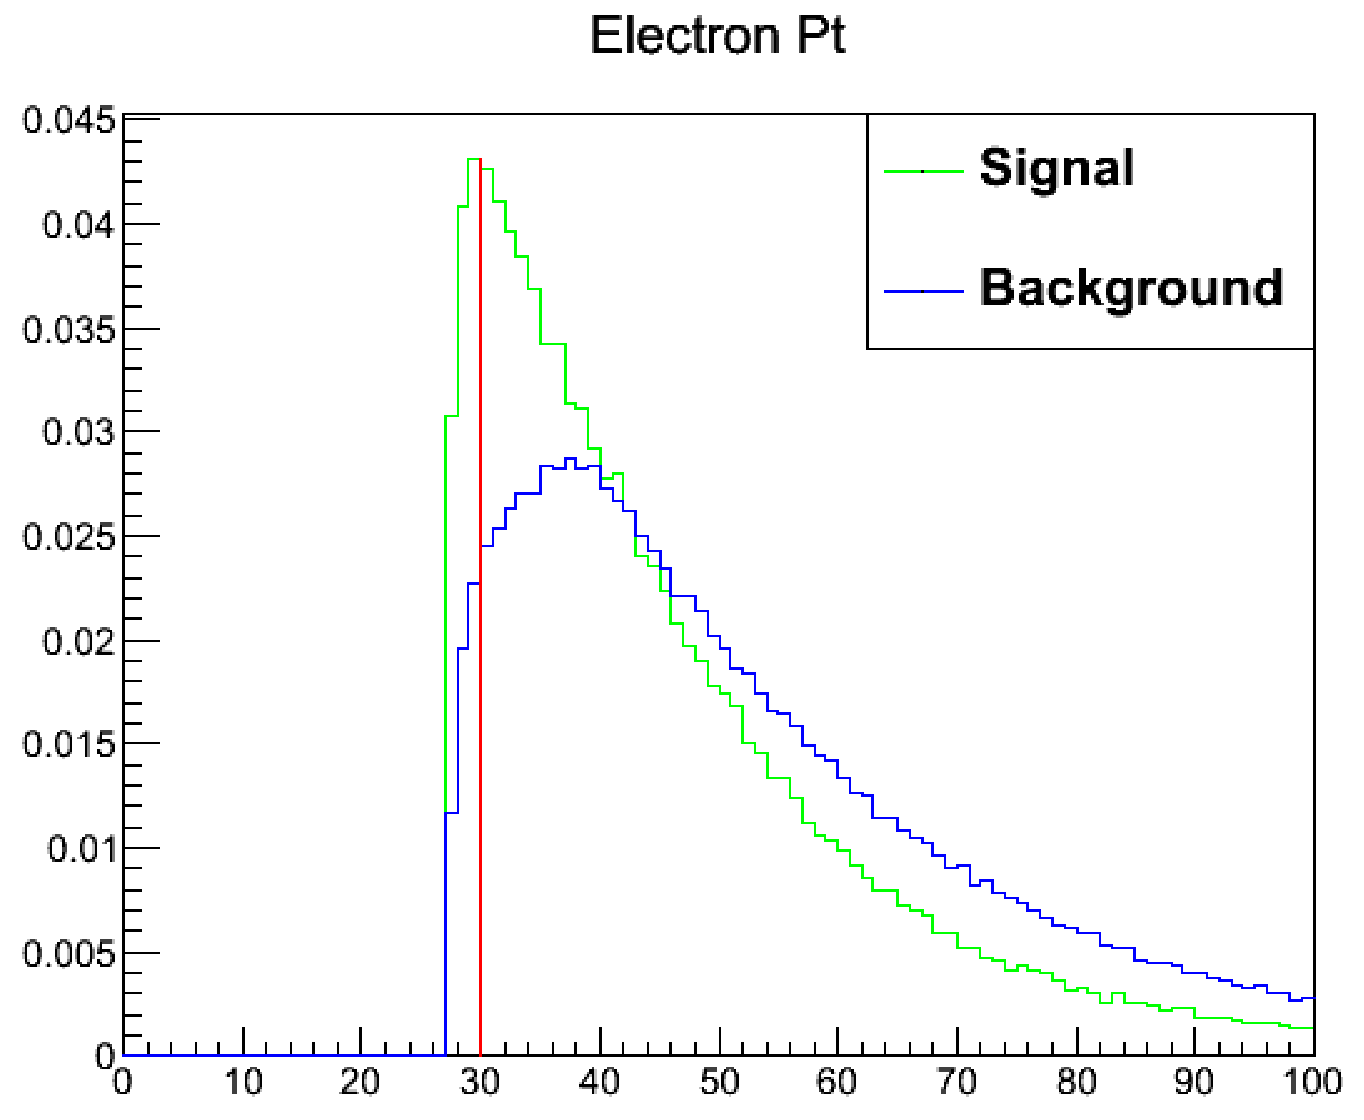
\includegraphics[width=0.95\textwidth]{\figpath/Chapter5/electronPt.png}
    \caption{Histograms of the electron \pt distribution where the gluon-gluon fusion signal is in green and the \Wjets background is in blue. The histograms are normalized to unit area. The red line show the cut on electron \pt where 5\% of the signal is lost.}
    \label{fig:electronPt_signal_loss}
\end{figure}

Beyond the lepton requirements, this analysis selected for any number of jets as long as they pass the selection criteria found in section~\ref{sec:jets}.
As the hadronic W decay will have at least two jets, that is the minimum number of jets needed to make it into the signal region, but we do not veto on additional jets which might come from ISR or FSR.
The requirement of the leading jet having a \ptgt{30}\gev was implemented to reduce the impact of the multijet background while minimally impacting the signal.
Besides the logical splitting of events based on lepton flavor, we also split events into three categories based on the number of jets in the event; exactly two jets, exactly three jets, and four or more jets.
As stated in section~\ref{sec:MET} we also require at least 25\gev of \VETslash.

Given that our signal has only one hadronic \W boson, we don't expect the $\W\rightarrow\bbbar$ branching fraction to contribute much to our signal.
However, we also want to remove as many \ttbar or single top events as possible, which are commonly associated with \cPqb quarks.
Thus we decided to veto events with b-tagged jets in order to reduce our backgrounds as much as possible.
An additional reason to do this is to keep the orthogonality between this analysis and another CMS analysis which was looking at the \VH production channel where \Hbb.
That analysis uses the same final state as this one, but requires two b-tagged jets~\cite{PhysRevD.89.012003}.
To prevent overlap, we only ever considered events with one or fewer b-tagged jets and then we separate the events into two categories based on the number of b-tags.
The zero b-tag events are used for signal extraction while the one b-tag events, which have a much larger impact from \ttbar and a higher \Hbb signal yield, are used for validation purposes and to check the volunteer signal contribution.

%Should I show the cut flow tables for 1-btagged category?

\section{MC Corrections}

Although a significant amount of work and time goes into making sure the MC simulation properly models the data, there can still exist discrepancies between the observed data and simulation
%there are still some corrections which must be made to the reconstructed objects or scale factors which must apply to weight each event in order to accurately mimic the behavior in data.
Often this occurs because the exact data taking conditions are not known in advance, like the pileup conditions that will exist.
Another reason the MC might not exactly mimic the data is that even state of the are generators are limited in their precision; much of the physics of hadronization is still unknown and hard physics processes can often only be computed up to NLO precision.
Data, on the other hand, contains all hadronization effects and all orders of precision.
I have already discussed some object specific corrections like the jet energy corrections, jet energy resolution, and \VETslash corrections in sections~\ref{sec:jets} and~\ref{sec:MET}.
For other discrepancies it is often necessary to reweight the full event rather than a specific object.

Broadly speaking these corrections can be separated into two categories: those which are common to all CMS analyses and those which are specific to this analysis.
The first category includes the b-tagging CSV discriminant weights and top quark \pt spectrum weights for the \ttbar simulation while the second category includes the weights for our multijet sample.
These event weights are applied after selecting for the events as they do not change the object kinematics.

\subsection{MC Pileup Reweighting}

Pileup is an important quantity as it can affect the reconstruction efficiency and even the observed kinematics of all the objects used in this analysis.
Up to this point it has been described as additional proton-proton interactions within an event, besides the interaction that produced the physics objects we are interested in studying.
There are several other properties of pileup which are worth noting.
I have so far either referred to pileup in a general sense or as relating to additional objects (tracks or energy) which might be found in the same bunch crossing as the event under study.
In reality there are two different categories of pileup.
There is indeed the pileup which comes from additional proton-proton interactions within the same bunch crossing, known as ``in-time'' pileup.
There is also energy from pileup added to objects because it was left in the sub-detectors from bunch crossings before or after the current one.
This is known as ``out-of-time'' pileup and comes about because the integration window of the sub-detectors can be larger than 25\unit{ns}.
An additional property is somewhat obvious in that the true number of proton-proton interaction within an event, $\mu$, is related to the instantaneous luminosity, which can vary over the course of data taking and even within a luminosity section (LS) period.
As a benchmark, the average number of proton-proton interactions per bunch crossing in 2012 was 21~\cite{LumiPublic}.

\begin{figure}[!hbt]
    \centering
    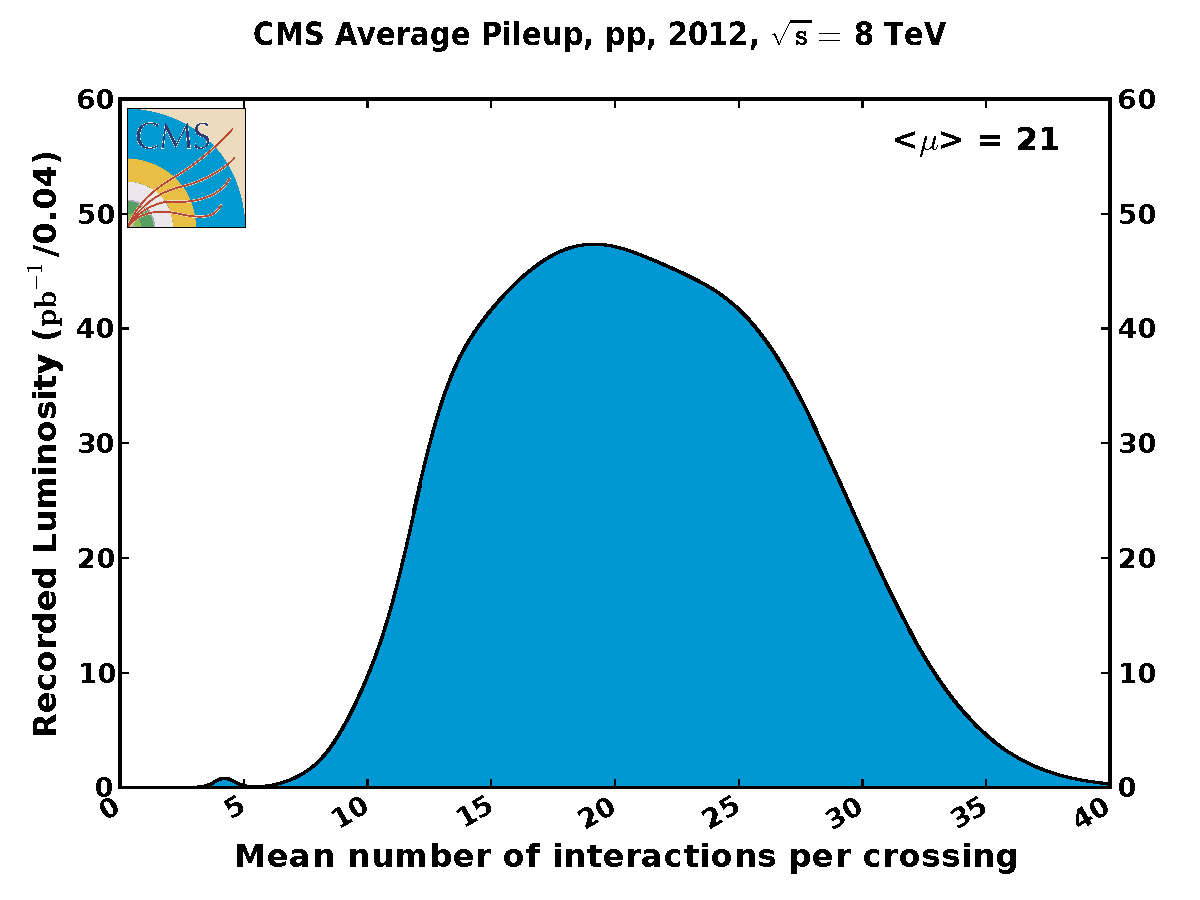
\includegraphics[width=0.95\textwidth]{\figpath/Chapter5/pileup_pp_2012.pdf}
    \caption{The mean number of interactions per bunch crossing in 2012. The min-bias cross section used for the calculation is 80\unit{mb}.}
    \label{fig:pileup_pp_2012}
\end{figure}

The MC samples used in CMS are usually generated before the data is taken and are thus created with an assumption of what the pileup conditions will look like in data.
A broad distribution of $\mu$ values, the number of min-bias pileup events overlaid on the hard scatter event, is generally chosen so as to cover all pileup conditions which might be experienced over the course of a data taking period.
Somewhat unsurprisingly the anticipated $\mu$ distribution rarely matches the one one observed in the data and thus the MC must be reweighted such that the $\mu$ distributions match~\cite{PileupStudiesTwiki}.
To generate a histogram for the average number of interactions per bunch crossing coming from data we make use of the approved pileupCalc tool provided by CMS.
This tool takes as input the total inelastic cross section $\sigma_{\text{inelastic}}=69.3\unit{mb}$\footnote{This is the CMS approved best fit value, not the theoretical value.}, a file in JSON format with every run number and luminosity section matched to a given average instantaneous luminosity and integrated luminosity for that given LS, and another JSON formatted file with the run numbers and LS used in the given analysis\footnote{This analysis uses the full 2012 ``golden'' JSON file called\\Cert\_190456-208686\_8TeV\_PromptReco\_Collisions12\_JSON.txt.}.
All of the MC samples used contain the same $\mu$ distribution scenario denoted by the ``S10'' notation in the dataset name.
The per event weights as a function of $\mu$ are created by dividing the normalized distribution from data by the normalized MC based distribution.
The weights are then applied to each MC event by looking up the weight for the mean number of pileup interactions used to generate that specific event~\cite{PileupWeightTwiki}. The distributions of pileup interactions in MC and data a well as the corresponding pileup weights can be seen in fig.~\ref{fig:pileup_reweighting}. Unfortunately, because the weights are not at unity, the statistical precision of the MC samples is reduced.
Fig.~\ref{fig:npv_comparison} shows the data to MC comparison of the N\textsubscript{PV} distribution before and after the pileup reweighting scheme has been applied.

\begin{figure}[!hbt]
    \centering
    \begin{subfigure}[t]{0.48\textwidth}
      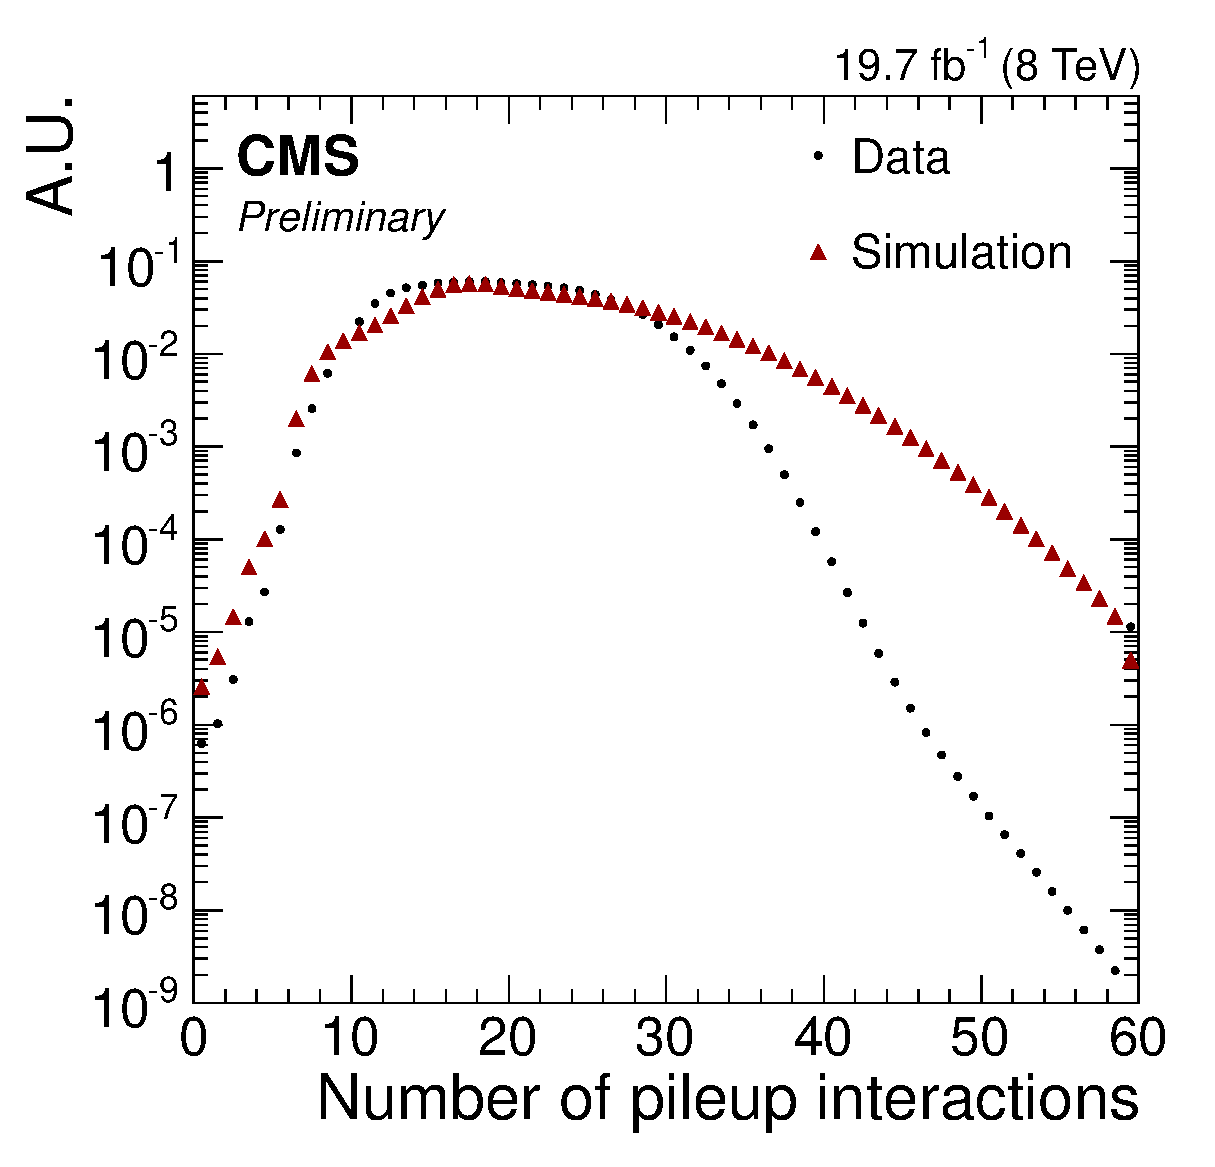
\includegraphics[width=0.95\textwidth]{\figpath/Chapter5/PileupDistribution.eps}
      \caption{}
      \label{fig:tnpu_distributions}
    \end{subfigure}
    \begin{subfigure}[t]{0.48\textwidth}
      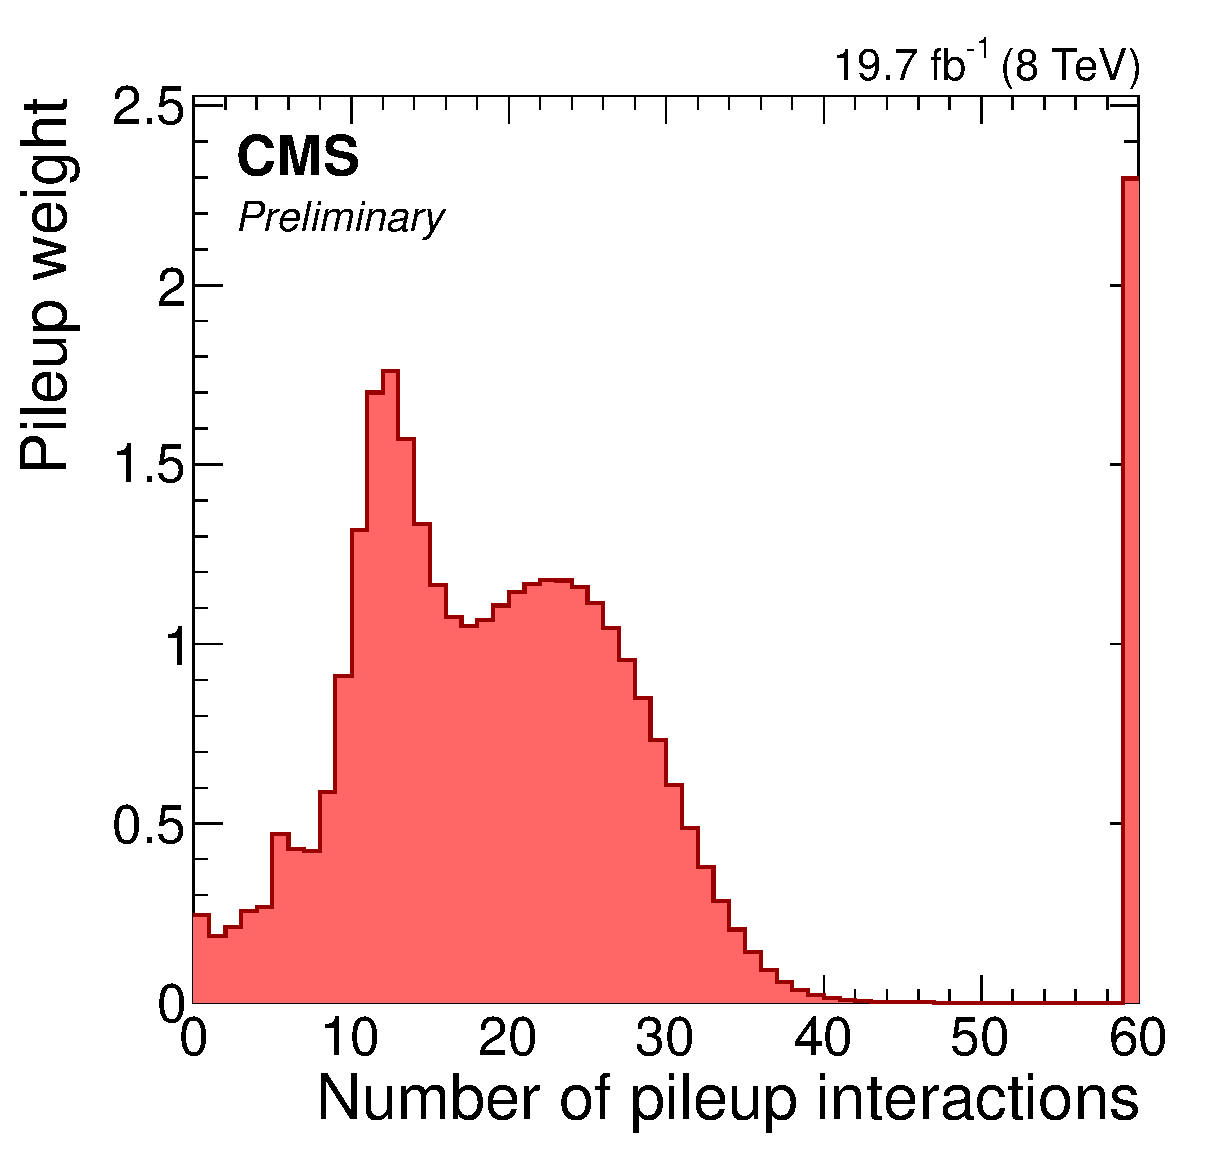
\includegraphics[width=0.95\textwidth]{\figpath/Chapter5/PileupWeights.eps}
      \caption{}
      \label{fig:pileup_weights}
    \end{subfigure}
    \caption{(a) Distributions of the number of pileup interactions in data and in simulation. (b) The derived pileup weights as a function of the number of interactions.}
    \label{fig:pileup_reweighting}
\end{figure}

\begin{figure}[!hbt]
    \centering
    \begin{subfigure}[t]{0.48\textwidth}
      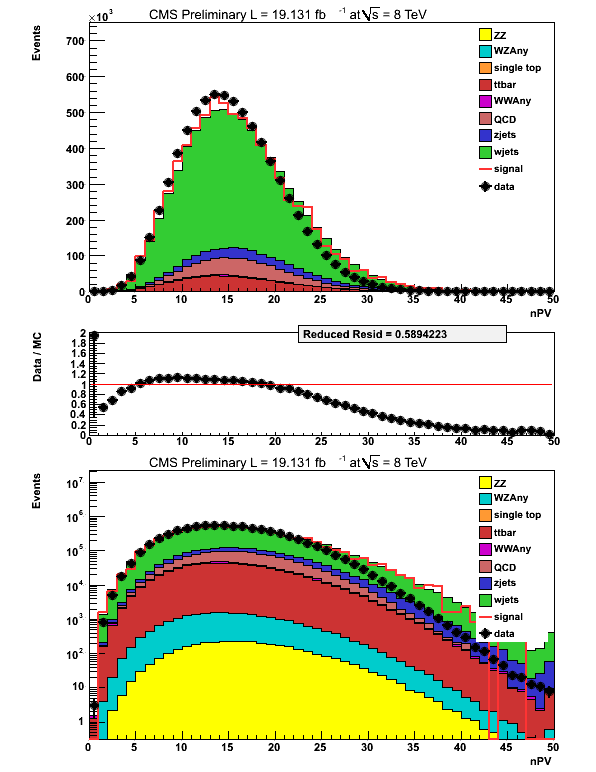
\includegraphics[width=\textwidth]{\figpath/Chapter5/nPV_noRW__comblep.png}
      \caption{}
      \label{fig:npv_no_pileup_reweight}
    \end{subfigure}
    \begin{subfigure}[t]{0.48\textwidth}
      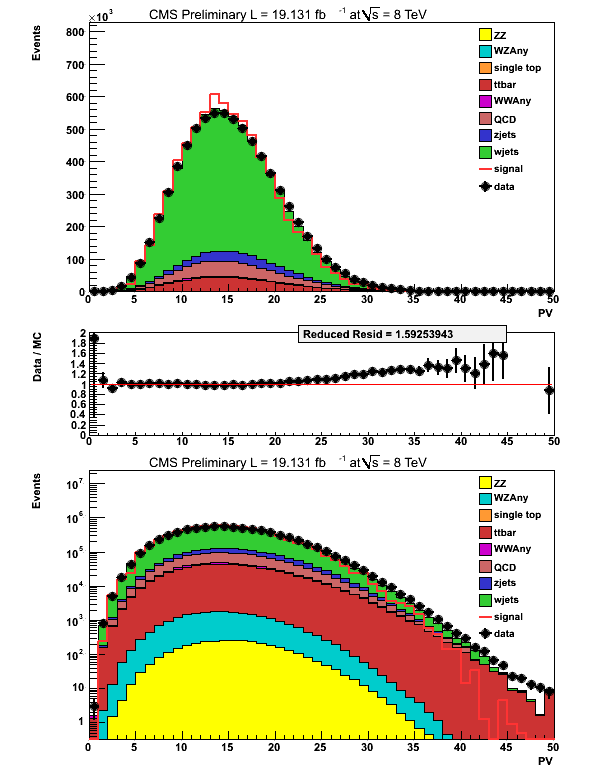
\includegraphics[width=\textwidth]{\figpath/Chapter5/nPV__comblep.png}
      \caption{}
      \label{fig:npv_pileup_reweight}
    \end{subfigure}
    \caption{Comparison of the number of primary vertices (N\textsubscript{PV}) in data and in MC (a) before the the pileup weights are applied and (b) after the weights are applied. These distributions correspond to the 19\fbinv collected during the 2012 data taking period and include both the electron and muon categories.}
    \label{fig:npv_comparison}
\end{figure}

\subsection{Jet Energy Corrections and Resolution}

The jet energy corrections and jet energy resolution scale factors make sure that the energy and resolution of the jets in MC matches those used in data and that the overall scale is correct.

\subsection{CSV Reweighting}
Ben: A comparison of the efficiency in data and Monte Carlo is shown in Figure 4.4. The scale factors shown in the figure are applied to the Monte Carlo to correct for the small differences. Scale factors are also applied to correct for differences in the mistag rate.

There is a reweighting of the events to correct the b-tag discriminant distributions and a reweighting to correct the \pt distributions of the \ttbar MC being used.

\subsection{TTbar Reweighting}
\subsection{\texorpdfstring{cos(theta$_l$)}{CosThetaL} Reweighting}
We also correct for a mis-modeling of the $\cos\left(\theta_{l}\right)$ angular variable

\subsection{QCD Reweighting}


Control region includes all of the same signal selection criteria, but only one jet.
This region is used for the normalization of the data-driven QCD sample.


The normalization of this background is found by doing a two component fit to the data, allowing only the \Wjets and QCD fractions to float.



\section{Data-to-MC Comparisons \& Yields}

Table~\ref{tab:FinalYields} shows the expected event yields in the signal region.

\begin{table}[htbp]
  \centering
  \noindent
  \small
    \begin{tabular}{|l|c|c|c|} \hline \hline
Process & $==$ 2 & $==$ 3 &  $\geq$4 \\ \hline
Diboson  & 39026.22 $\pm$ 197.55 & 12612.58 $\pm$ 112.31 & 3485.46 $\pm$ 59.04 \\
$W$+jets  & 3271138.31 $\pm$ 1808.63 & 726384.44 $\pm$ 852.28 & 187723.52 $\pm$ 433.27 \\
$Z$+jets  & 272583.99 $\pm$ 522.10 & 69588.32 $\pm$  263.80 & 19937.11 $\pm$ 141.20 \\
$t\bar{t}$  & 20005.51 $\pm$ 141.44 & 24748.61 $\pm$ 157.32 & 27686.99 $\pm$ 166.39 \\
Single $t$ & 16318.38 $\pm$ 127.74 & 7096.2 $\pm$ 84.24 & 3036.83 $\pm$ 55.11 \\
Multi-Jet  & 450503.85 $\pm$ 671.20 & 119248.8 $\pm$ 345.32 & 33681.6 $\pm$ 183.53 \\ \hline
Tot Bkg & 4069576.26 $\pm$ 2017.32 & 959678.95 $\pm$ 979.63 & 275551.51 $\pm$ 524.93 \\\hline \hline
ggH, H$\rightarrow$WW $M_{H}=125$  & 548.49 $\pm$ 23.42 & 210.97 $\pm$ 14.52 & 79.87 $\pm$ 8.94 \\
qqH, H$\rightarrow$WW $M_{H}=125$  & 106.34 $\pm$ 10.31 & 52.53 $\pm$ 7.25 & 17.47 $\pm$ 4.18\\
WH\_ZH\_TTH, H$\rightarrow$WW $M_{H}125$ & 124.51 $\pm$ 11.16 & 77.97 $\pm$ 8.83 & 42.95 $\pm$ 6.55\\
WH\_ZH\_TTH, H$\rightarrow$ZZ $M_{H}125$ & 8.27 $\pm$ 2.88 & 4.4 $\pm$ 2.10 & 2.25 $\pm$ 1.50\\
WH, H$\rightarrow$b$\bar{b}$ $M_{H}125$ & 40.2 $\pm$ 6.34 & 12.63 $\pm$ 3.55 & 3.39 $\pm$ 1.84\\
TTH, H$\rightarrow$b$\bar{b}$ $M_{H}=125$ & 0.53 $\pm$ 0.73 & 1.14 $\pm$ 1.07 & 3.14 $\pm$ 1.77 \\ \hline
Total Signal & 828.33 $\pm$ 28.78 & 359.64 $\pm$ 18.96 & 149.07 $\pm$ 12.21 \\ \hline
    \end{tabular}
    \caption{Expected event yield in the signal region after combining the lepton channels.}
    \label{tab:FinalYields}
\end{table}

\section{Multivariate Analysis: Kinematic Boosted Decision Tree}
Rishi Thesis pages 76-79
\subsection{Kinematic Variable Selection}
\subsection{BDT Input Optimization}
\subsection{BDT Parameter Optimization}
\subsection{Signal Extraction Methods}

\section{Matrix Element Analysis}
Matrix Element Method (MEM)

\begin{comment}
Table~\ref{tab:FinalYields} clearly shows that the total signal, in every channel, is smaller than even the statistical uncertainty of the background.
A cut and count experiment will not lead to any significant results.
The previous \HWWlnujj analyses have performed a fit to sensitive distributions like the 4-body mass, the mass of the two jet plus lepton plus \ETslash system.
However, this approach only includes a small amount of information available, leaving out additional sensitive kinematic distributions.
It is also felt that a BDT analysis using only kinematic variable would be sub-optimal because shallow classifiers are not robust against non-linear correlations and are only as good as the input variables.

Instead, this analysis uses a matrix element method (MEM), which starts from the differential cross section calculation from quantum field theory to classify how likely and event is to come from a given process~\cite{Canelli2003,Dong2008}.
The probability $P\left(x;\alpha\right)=P_{evt}$ of a signal is proportional to the differential production cross section, where $\alpha$ is the parameter we wish to measure and x is a set of physical variables.
This is true if the detector resolution is sufficiently small and the beam energies are well known, as it is in the case of CMS.
In general the differential cross section can be written as~\cite{Olive:2016xmw}:
\begin{equation}\label{eq:differential_production_cross_section}
d\sigma=\frac{\left(2\pi\right)^{4}|\mathcal{M}|^{2}}{4\sqrt{\left(q_{1}\cdot{q_{2}}\right)^{2}-m_{q_{1}}^{2}m_{q_{2}}^{2}}}d\Phi_{n}\left(q_{1}+q_{2};p_{1},...,p_{n}\right)
\end{equation}
where $|\mathcal{M}|$ is the Lorentz invariant matrix element (ME); $q_{1}$, $q_{2}$ and $m_{1}$, $m_{2}$ are the 4-momenta and masses of the incident particles; $p_{i}$ are the 4-momenta of the final state particles; and $d\Phi_{n}$ is the n-body phase space.
The phase space term is written as:
\begin{equation}
d\Phi_{n}\left(q_{1}+q_{2};p_{1},...,p_{n}\right)=\delta^{4}\left(q_{1}+q_{2}-\sum_{i=1}^{n}p_{i}\right)\prod_{i=1}^{n}\frac{d^{3}p_{i}}{\left(2\pi\right)^{3}2E_{i}}
\end{equation}
After accounting for unmeasured or mis-measured particles and normalizing to the total cross section to form an event probability, equation~\ref{eq:differential_production_cross_section} becomes:
\begin{equation}
P(x;\alpha)=\frac{1}{\sigma}\int2\pi^{4}|\mathcal{M}|^{2}\frac{f\left(x_{1}\right)}{|E_{q_{1}}|}\frac{f\left(x_{2}\right)}{|E_{q_{2}}|}W\left(y,x\right)d\Phi_{4}dE_{q_{1}}dE_{q_{2}}
\end{equation}
where $f\left(x_{i}\right)$ are the PDFs, $x_{i}=E_{q_{i}}/E_{beam}$ is the fraction of the proton momentum carried by the incident parton $i$, and $W\left(y,x\right)$ is the transfer function mapping measured jet energies $x$ to the parton energies $y$ (accounts for the jet resolution of CMS).

Fifteen probabilities $P(x;\alpha)$, corresponding to the leading order diagrams of the major background and signal processes, are computed for each event. 
This computation is by far the most time consuming aspect of this analysis, consuming $\sim$12 million CPU hours.
The information contained in these 15 probabilities must be combined in order to discriminate signal from background.
\end{comment}


\subsection{Differential Cross Section}
\subsection{Parton Distribution Functions and Phase Space}
\subsection{Transfer Functions}
\subsection{Combinatorial Considerations}
\subsection{Numerical Integration}
\subsection{Matrix Element Computation}
\subsection{Standalone BDT}
\subsection{Combined BDT}

\begin{comment}
In order to combine the complimentary information from the kinematic variables and the MEs, with the purpose of discriminating a Higgs event from a background event, we used several Boosted Decision Trees (BDTs).
An initial BDT was computed which combined the information from 15 of the computed MEs.\footnote{A BDT was used rather than combining the ME into a likelihood as in the Matrix Element Likelihood Analysis (MELA) used by H$\rightarrow$ZZ$\rightarrow$4l or using some basic ratios of signal over background probabilities as was done by CDF.}
This gives a less discriminating shallow network the ability to create a better performing network because the inputs are already non-linear variables.
The output of this BDT, along with several carefully selected kinematic variables, is then used as the input to a new BDT in order to combine all of this complimentary information.
While it may seem that the MEs should encode all of the event information perfectly, only the leading MEs were used and the permutations of the jets and partons degrades the discrimination power of the MEs.
The combined BDT has more discrimination power than either the MEs or the kinematic variables alone. 

A distribution of the BDT discriminant is produced for every signal, background, and data sample and then passed to the RooStats-based Higgs Combine Tool~\cite{CombineToolTwiki} to compute limits on the Higgs signal strength.
Given that this analysis has a relatively high number of events in the expected yields we make use of the asymptotic method\footnote{If there had been a lower number of expected events we may have needed to use the full frequentist method rather than the asymptotic method.} for limit setting along with the CL\textsubscript{s} test statistic~\cite{Read:2002hq}.
Using an Asimov dataset an expected 95\% upper confidence level is obtained and shown in figure~\ref{fig:limits} (left).
\end{comment}

original bin width 0.02 [-1,1]
bin must have background events
stat error must be less than 10\%
bins merged left to right until all bins meet this criteria
limited or no background in a bin would lead to an inflated signal significance if data, but no background

\section{Systematic Uncertainties}
TURN THESE SUBSECTIONS INTO BOLDED PARAGRAPH HEADERS

\subsection{Jet Energy Scale}
\subsection{Lepton Selection and Trigger Efficiency}
\subsection{W+jets Shape Uncertainties}
\subsection{Pileup Weights}
In order to assess the effect of a systematic uncertainty due to choice of $\sigma_{\text{inelastic}}=69.3\unit{mb}$, a $\pm$7\% variation was used.
\subsection{CSV Weights}
\subsection{Top \texorpdfstring{$p_{T}$}{pT}}
\subsection{LHC Luminosity}
\subsection{Sample Cross Sections}
\subsection{MET Uncertainty }
\subsection{QCD \texorpdfstring{$\eta$}{eta} Weights Uncertainty}
\subsection{Summary of Systematics}

\begin{comment}
Given that this is a shape analysis, it is important to consider systematic uncertainties that may change the expected yields (rate changes), the shape of the discriminating variable, or both.
This analysis considers all three of these, but decouples the rate and shape changes during limit setting.
Table~\ref{tab:ListOfSystematics} summarizes all of the systematic uncertainties considered for this analysis.
Changes to the limits greater than 1\% come from the scheme used to reweight the $\eta$ distribution in the QCD sample, the jet energy scale, the $\cos\left(\theta_{l}\right)$ weights, and the lepton efficiency uncertainty.
There will be much more detail on each of the systematics in the thesis.

\begin{table}[htbp]
  \centering
  \noindent
  \small
    \captionsetup{width=.85\textwidth}
    \caption*{Systematic Uncertainties for H$\rightarrow$WW$\rightarrow$l$\nu$jj Analysis}
    \begin{tabular}{|l|c|c|c|} \hline
Uncertainty & Rate (Y/N) 2 & Shape (Y/N) & Comments \\ \hline
$Q^{2}$ Scaling & Y & Y & W+jets MC only \\ \hline
ME/PS Matching & Y & Y & W+jets MC only \\ \hline
Background xSec & Y & N & All background samples \\  \hline
Signal xSec & Y & N & All signal MC samples \\  \hline
Luminosity & Y & N & All samples \\  \hline
MC Pileup reweighting & Y & N & All MC samples \\  \hline
Trigger Efficiency & Y & N &  All MC samples\\  \hline
Lepton Selection Efficiency & Y & N & All MC samples\\  \hline
JES Uncertainties & Y & Y & All MC samples \\  \hline
Met Uncertainty & Y & N & All samples\\  \hline
CSV Reshaping & Y & N &  All MC samples\\  \hline
Top Pt-reweighting & Y & Y &  TTbar MC only\\  \hline
QCD $\eta$ Weight & Y & Y & QCD shape, W+jets and QCD rate \\ \hline
$\cos\left(\theta_{l}\right)$ Weight & N & Y & W+jets MC only \\ \hline
    \end{tabular}
    \caption{List of all systematic uncertainties applied in analysis, whether that uncertainty has a rate or shape component to it, and which samples is is applied to.}
    \label{tab:ListOfSystematics}
\end{table}
\end{comment}